\chapter{Projeto de Pesquisa}\label{Cap:Projeto de Pesquisa}

%  https://bdm.unb.br/bitstream/10483/27583/1/2020_GabrielCampos_LucasMoutinho_tcc.pdf

Neste capítulo é apresentada a proposta contida neste trabalho. O capítulo irá se desdobrar a partir do problema encontrado e proporá uma solução para sua realização. Adiante, irá expor a sua implementação em detalhes, tratando conhecimentos mais específicos que não estejam elucidados ao longo dos capítulos anteriores e conjecturando sobre possíveis aplicabilidades deste trabalho em áreas diversas. Finalmente, as atividades propostas para este projeto de pesquisa, juntamente com um cronograma de acompanhamento, de acordo com o estabelecido pelo Programa de Pós-Graduação em Informática da Universidade de Brasília (PPGI/UnB) para a obtenção do título de Mestre.\\

% ==========================================================================================
\section{Motivação}

Independente de formação enquanto profissionais de saúde mental, é natural que consigamos atribuir alguma espécie de métrica para comparar duas instâncias de uma mesma emoção que tenhamos sentido. Parece trivial quando atestamos que, entre dois momentos experimentando uma mesma emoção, um foi mais ou menos intenso do que o outro, ou até que ambos tiveram a mesma intensidade. Portanto, somos capazes de identificar emoções, quantificar sua intensidade e calcular uma distância para poder efetuar essa comparação.

Conforme visto, trabalhos de \textit{ML} aplicados ao reconhecimento de emoções na fala vêm sendo publicados - ao menos - desde o início da década de 90 (1990), e se tornam menos frequentes quando buscamos por tarefas mais especializadas.

Não tendo encontrado ocorrência na literatura, este trabalho se propõe a responder a seguinte pergunta: É possível realizar uma tarefa de aprendizado de máquina para inferir a intensidade das emoções na voz em português?

% ==========================================================================================
\section{\textit{BRAVO: Brazilian-portuguese Emotional Intensity Recognition Assistant for Voice}}

% ------------------------------------------------------------------------------------------
\subsection{Visão Geral}

Na Figura \ref{fig:visaogeralproposta} é apresentada uma visão geral da proposta. Conforme a imagem, três etapas principais são necessáiras para o reconhecimento da intensidade das emoções: (A) Aquisição dos dados; (B) Extração de características; e (C) Classificação da intensidade.

\begin{figure}[!h]
\centering
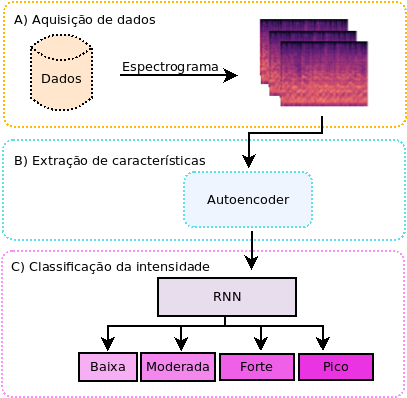
\includegraphics[width=0.75\textwidth]{imagens/arquitetura-visao-geral.png}
\caption{\label{fig:visaogeralproposta}Visão geral da proposta}
\end{figure}

A primeira etapa (A) lida com a obtenção dos dados que serão utilizados no projeto e da sua conversão para uma interpretação passível de utilização por modelos de aprendizagem de máquina. Podemos descrever os dados como um conjunto de registros rotulados que serão utilizados para treinamento, teste e validação dos modelos implementados na proposta.

A segunda etapa (B) lida com a extração de características dos dados convertidos. Essas \textit{features} serão obtidas através de um modelo não supervisionado para a redução de dimensionalidade e posteriormente utilizadas como entrada de um modelo supervisionado de classificação da intensidade da emoção.

A terceira e última etapa (C) é responsável pela inferência da intensidade. O modelo recebe as \textit{features} obtidas na etapa anterior e realiza o treinamento e testagem do modelo de classificação de acordo com quatro classes possíveis: (i) Baixa; (ii) Moderada; (iii) Forte; e (iv) Pico de intensidade.

% ------------------------------------------------------------------------------------------
\subsection{Aquisição dos dados}

O primeiro passo para tarefas de \textit{machine learning} que envolvem \textit{SER} costuma ser a aquisição dos dados que serão utilizados pelo modelo. Em virtude do escopo da proposta, necessitamos de um \textit{dataset} em português que possua as classes desejadas: Emoção e intensidade.

Até o momento da escrita deste tabalho, não sabemos de nenhum \textit{dataset} que seja ideal (idioma, emoções e intensidade) para esta proposta. Então, conforme descrito na seção \ref{section:basesdedados}, este trabalho utilizará duas bases de dados: VERBO \cite{12.21} e VIVAE \cite{16}.

O primeiro \textit{dataset}, VERBO, é composto por vocalizações verbais, acomodando todos os fonemas da língua portuguesa, com exemplos para seis emoções básicas (alegria, nojo, medo, raiva, surpresa, tristeza) e um estado emocional denominado de neutro.

O segundo, VIVAE, é composto por vocalizações não verbais distribuidas em seis classes (conquista, prazer sexual, surpresa positiva, raiva, medo e dor física), com exemplos em quatro intensidades (baixa, moderada, fote e pico de intensidade). Graças a fusão de domínios \cite{49}, conseguimos o cenário da Tabela \ref{table:datasetideal}.

Assim, sejam os dois \textit{datasets} VERBO e VIVAE, de modo que VERBO é constituído por pares \{amostra, classe\} e VIVAE por pares \{amostra, classe, intensidade\}, onde as classes são a emoção atribuída àquela amostra, e a intensidade é o rótulo da intensidade da classe daquela amostra. Vamos representar as amostras do VERBO por $X_{VERBO}$ e do VIVAE por $X_{VIVAE}$.

\begin{table}[!h]
\centering
\label{table:datasetideal}
\caption{Atributos dos datasets VERBO, VIVAE, ideal e da fusão de domínios}
\begin{tabular}{l|cccc|}
\cline{2-5}
 & \multicolumn{4}{c|}{Datasets} \\ \hline
\multicolumn{1}{|l|}{Atributos} & \multicolumn{1}{c|}{VERBO} & \multicolumn{1}{c|}{VIVAE} & \multicolumn{1}{c|}{Ideal} & Data Fusion(VERBO,VIVAE) \\ \hline
\multicolumn{1}{|l|}{Idioma} & \multicolumn{1}{c|}{X} & \multicolumn{1}{c|}{} & \multicolumn{1}{c|}{X} & X \\ \hline
\multicolumn{1}{|l|}{Emoções} & \multicolumn{1}{c|}{X} & \multicolumn{1}{c|}{X} & \multicolumn{1}{c|}{X} & X \\ \hline
\multicolumn{1}{|l|}{Intensidade} & \multicolumn{1}{c|}{} & \multicolumn{1}{c|}{X} & \multicolumn{1}{c|}{X} & X \\ \hline
\end{tabular}
\end{table}

Seja $Y_{VERBO}$ o conjunto das classes (emoções) $y_i \forall x_i \in X_{VERBO}$, analogamente para $Y_{VIVAE}$, vamos definir $Y = Y_{VERBO} \bigcap Y_{VIVAE}$. Vamos definir por por $Z$ o conjunto das intensidades. Sabemos das Tabelas \ref{table:vivaeintensidade} e \ref{table:totalporclasse} que

\begin{itemize}
    \item $Y = \{alegria, medo, raiva, supresa\}$
    \item $Z = \{baixa, moderada, forte, pico\}$
\end{itemize}

\begin{figure}[!h]
\centering
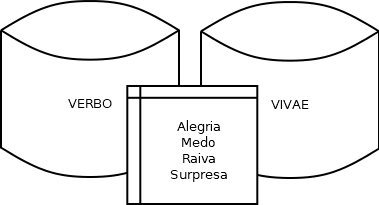
\includegraphics[width=0.40\textwidth]{imagens/p-yverbointeryvivae.png}
\caption{\label{fig:yverbointeryvivae}Interseção entre rótulos de emoções de VERBO e VIVAE}
\end{figure}

Vamos redefinir $X_{VERBO} = \{x_i \mid y_i \in Y\}$, analogamente para $X_{VIVAE}$, e vamos definir nosso domínio $X = X_{VERBO} \bigcap X_{VIVAE}$, assim

\begin{itemize}
    \item $\forall x_i \in X, \exists y_i \in Y$ tal que  $y_i$ é a classe de $x_i$
    \item $\forall x_j \in X_{VIVAE}, \exists z_j \in Z$ tal que  $z_j$ é a intensidade de $x_j$
\end{itemize}

Ao realizar tarefas de \textit{DL}, precisamos transformar os dados de entrada em um formato passível de ingestão pelos modelos. Os arquivos \textit{.wav} de $X$ serão lidos e iremos gerar seus respectivos \textit{Mel-spectrograms}, convertendo o sinal de áudio ao longo do tempo para uma representação do sinal no domínio da frequência, que será utilizada pelos modelos. Então, teremos um mapa $M(x_i): espectrograma_i$.

\begin{figure}[!h]
\centering
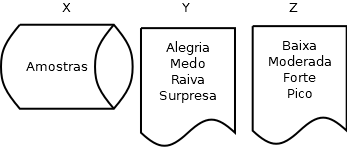
\includegraphics[width=0.5\textwidth]{imagens/p-dominios-contradominos.png}
\caption{\label{fig:dominioscontradominios}Domínio e contradomínios}
\end{figure}

% ------------------------------------------------------------------------------------------
\subsection{Extração de características}

De posse do mapa $M(x_i)$, podemos prosseguir para a etapa de extração de características. Apesar da representação visual, o espectrograma é dado por um vetor de alta dimensionalidade. Uma vez que $X$ é formado por dados de \textit{datasets} diferentes, buscamos uma forma de extrair características relevantes com boa capacidade de generalização ao ser aplicada em ambos $X_{VERBO}$ e $X_{VIVAE}$.

Redes neurais constituem uma boa ferramenta para tarefas de \textit{SER}. CNNs como \textit{feature extractors}, mais ainda \textit{Autoencoders}, podem criar uma representação de qualidade com dimensionalidade reduzida em seu espaço latente, enquanto \textit{DNNs} encotram espaço na literatura como bons discriminadores ou classificadores.

Vamos construir um \textit{Autoencoder} ($AE$) que tenta reproduzir uma função identendide. Por definição, um \textit{Autoencoder} é composto por uma função \textit{encoder} ($f_e$) e uma função $decoder$ ($f_d$), de modo que $AE: M \rightarrow M'$ faça

\begin{equation}
    AE(x) = f_d(f_e(x)) = x' \approx x
\end{equation}

\begin{figure}[!h]
\centering
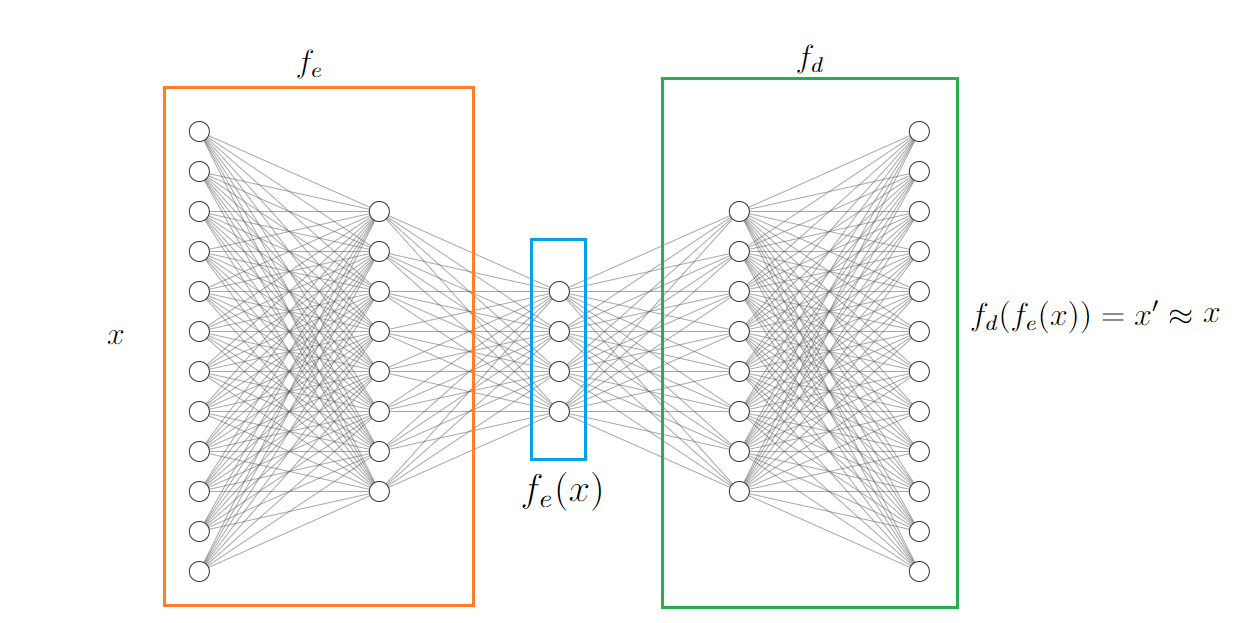
\includegraphics[width=0.9\textwidth]{imagens/p-autoencoder.png}
\caption{\label{fig:treinamentoae}Treinamento do \textit{AE}}
\end{figure}

O modelo $AE$ será treinado em $X$, e em seu espaço latente teremos uma representação do dado de entrada com a dimensionalidade reduzida, preservando suas características de maneira suficiente para que possa ser reconstruído ($x'$) ao aplicar a função de \textit{decoding}.

Após o treinamento, vamos separar $X_{VIVAE}$ em três partes com proporções $0,8$, $0,1$ e $0,1$, que irão formar as amostras de treino ($X_{VIVAE_{treino}}$), teste ($X_{VIVAE_{teste}}$) e validação ($X_{VIVAE_{validacao}}$), respectivamente, do modelo supervisionado $j$ que iremos construir a seguir.

% \subsubsection{Design da arquitetura}

% ------------------------------------------------------------------------------------------
\subsection{Classificação da Intensidade}

Através do modelo de Russel sabemos que que é possível dispor as emoções em função da valência (prazer ou desprazer) e da ativação (vigor ou quietude) \cite{27}. Plutchik decompõe as emoções básicas de acordo com a intensidade, chegando a emoções compostas, formadas a partir de duas emoções com intensidades menores.

Ao longo do Capítulo \ref{Cap:Trabalhos Relacionados}, observamos trabalhos relacionados, desafios pertinentes à pesquisa e o estado da arte na área de estudo deste trabalho, que se diferencia dos pares por, além de ser um dos poucos trabalhos a lidar com o idioma português, também aborda a questão da intensidade da emoção.

Sabemos da relevância que \textit{features} espectrais carregam sobre a vocalização e vimos formas para avaliar o desempenho dos modelos, como o \textit{F1-Score}. Para a etapa de classificação da intensidade, vamos construir e treinar um modelo supervisionado $j$ (e.g.: \textit{CNN-LSTM}) que recebe como \textit{input} o \textit{encoding} do \textit{mel-spectrogram} dos $x_i \in X_{VIVAE_{treino}}$.

Este modelo será construído para classificar a intensidade da emoção de forma direta. Uma vez que os $x_i \in X_{VIVAE_{treino}}$ têm correspondentes em $Z$, contra domínio das intensidades, então, $j: M \rightarrow Z$, é tal que

\begin{equation}
    j(f_e(m)) = z
\end{equation}

\begin{figure}[!h]
\centering
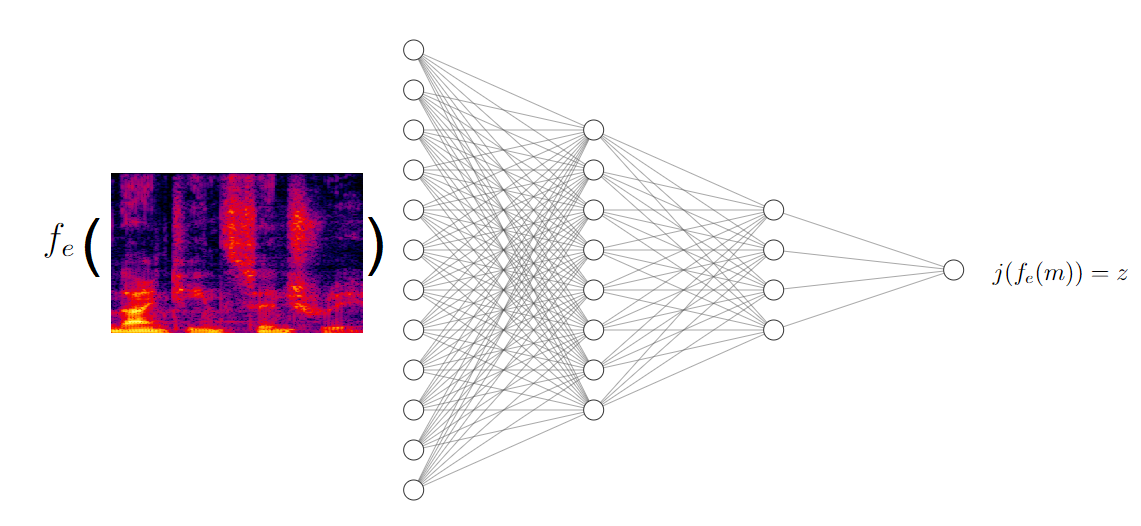
\includegraphics[width=1.0\textwidth]{imagens/p-supervisionado.png}
\caption{\label{fig:jsupervisionado}Modelo supervisionado $j$}
\end{figure}

Por ser tratar de um modelo supervisionado, podemos aplicar as méricas descritas em \ref{sec:metricas}, utilizando $X_{VIVAE_{validacao}}$ e $X_{VIVAE_{teste}}$ para testar e validar seus resultados. Uma vez que o desempenho de $j$ seja satisfatório, vamos aplicar $j$ em $X_{VERBO}$, obtendo $Z' = \{z'{_i} = j(x_i), \forall x_i \in X_{VERBO}\}$, que serão os resultados para as intensidades das emoções de $X_{VERBO}$.

% \subsubsection{Design da arquitetura}

% ------------------------------------------------------------------------------------------
\subsection{Validação}

Como não existe correspondência entre $X_{VERBO} \rightarrow Z$, não podemos validar imediatamente as intensidades $z'$. Sabendo as intensidades reais $z_i$ dos $x_i \in X_{VIVAE}$, podemos agregar as features e intensidades, formando vetores, $v_i, u_i$, onde

\begin{itemize}
    \item $v_i = [f_e(m_i), y_i, z_i]$, onde $x_i \in X_{VIVAE}$
    \item $u_i = [f_e(m_i), y_i, j(m_i) = z'_i]$, onde $x_i \in X_{VERBO}$
\end{itemize}

Portanto, devemos ter vetores $u,v$ que contêm atributos representativos de características relativas a emoção, sua classe e a intensidade dessa emoção.

Algoritmos não supervisionados como \textit{PCA} e \textit{K-means} podem atuar como formadores de \textit{clusters} para avaliar o desempenho de geração de dados sintéticos.

Podemos então aplicar técnicas de clusterização (e.g.: \textit{PCA}) para investigar se os vetores com classe ($y$) e intensidade ($z$) são agrupáveis de forma coerente com base em suas características $y, z$ e verificar a validade de $j$ em $X_{VERBO}$.

% Uma forma de aferir o desempenho da clusterização é ...

\begin{figure}[!h]
\centering
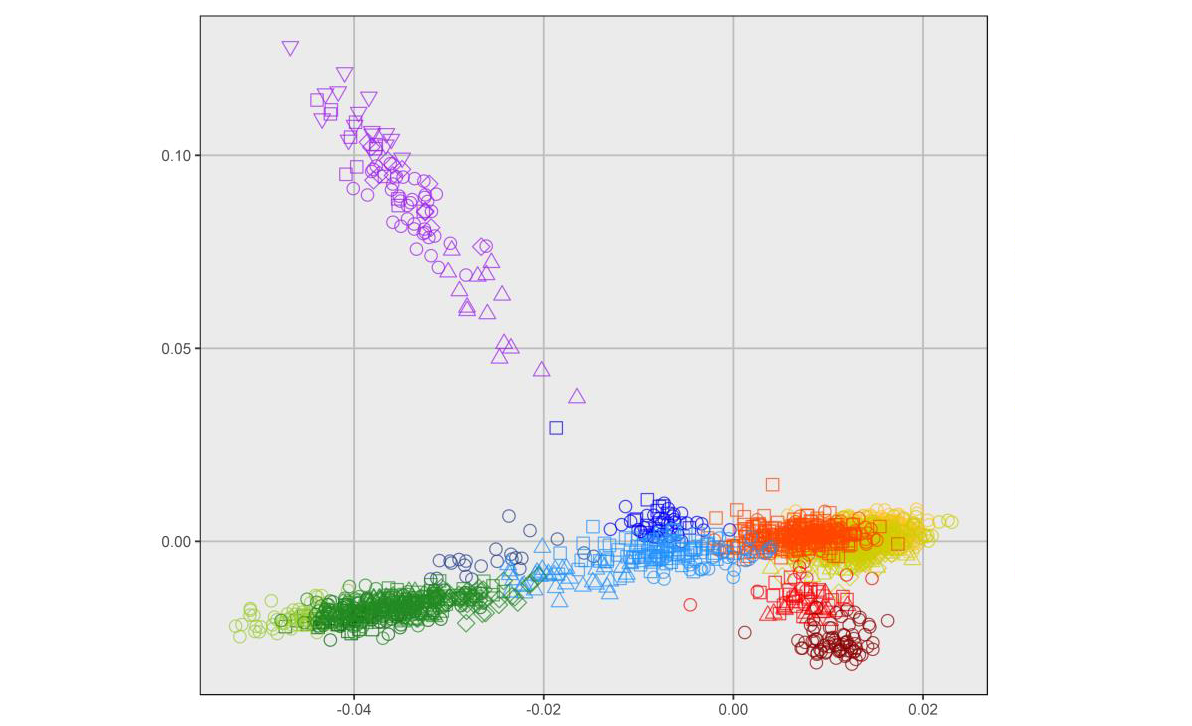
\includegraphics[width=1.0\textwidth]{imagens/p-naosupervisionado.png}
\caption{\label{fig:clusterizacaoresults}Exemplo de clusterização de resultados}
\end{figure}

% ------------------------------------------------------------------------------------------
% \section{Aplicabilidade da solução}

% ==========================================================================================
\section{Plano de Trabalho e Cronograma}

Esta seção apresenta as atividades propostas para este projeto de pesquisa, juntamente com um cronograma de acompanhamento. Planeja-se finalizar o projeto em dois anos de atividades. Abaixo, temos enumeradas as atividades necessárias para a conclusão do Programa de Pós-Graduação em Informática da Universidade de Brasília (PPGI/UnB) e obtenção do título de Mestre. A Tabela \ref{table:cronogramaproposta} apresenta o cronograma de atividades deste plano de trabalho.\\

Atividades:

\begin{enumerate}
    \item Obtenção dos créditos obrigatórios exigidos pelo programa de mestrado;
    \item Obtenção da certificação de proficiência em idioma Inglês;
    \item Revisão da literatura, fundamentação teórica e apresentações;
    \item Redação e exame da qualificação;
    \item Planejar, realizar e analisar os experimentos;
    \item Publicação dos resultados;
    \item Redação da dissertação e defesa do mestrado.
\end{enumerate}

\begin{table}[!h]
\centering
\label{table:cronogramaproposta}
\caption{Cronograma proposto de atividades, onde \textbf{X} representa atividades finalizadas e \textbf{O} representa atividades a desenvolver}
\label{tab:my-table}
\begin{tabular}{ccccccccc}
\cline{3-9}
 & \multicolumn{1}{c|}{} & \multicolumn{7}{c|}{Atividade no trimestre} \\ \hline
\multicolumn{2}{|c|}{Período} & \multicolumn{1}{c|}{1} & \multicolumn{1}{c|}{2} & \multicolumn{1}{c|}{3} & \multicolumn{1}{c|}{4} & \multicolumn{1}{c|}{5} & \multicolumn{1}{c|}{6} & \multicolumn{1}{c|}{7} \\ \hline
\multicolumn{1}{|c|}{\multirow{2}{*}{2022}} & \multicolumn{1}{c|}{3o trimestre} & \multicolumn{1}{c|}{X} & \multicolumn{1}{c|}{} & \multicolumn{1}{c|}{} & \multicolumn{1}{c|}{} & \multicolumn{1}{c|}{} & \multicolumn{1}{c|}{} & \multicolumn{1}{c|}{} \\ \cline{2-9} 
\multicolumn{1}{|c|}{} & \multicolumn{1}{c|}{4o trimestre} & \multicolumn{1}{c|}{X} & \multicolumn{1}{c|}{X} & \multicolumn{1}{c|}{X} & \multicolumn{1}{c|}{X} & \multicolumn{1}{c|}{X} & \multicolumn{1}{c|}{} & \multicolumn{1}{c|}{} \\ \hline
\multicolumn{1}{|c|}{\multirow{4}{*}{2023}} & \multicolumn{1}{c|}{1o trimestre} & \multicolumn{1}{c|}{X} & \multicolumn{1}{c|}{} & \multicolumn{1}{c|}{O} & \multicolumn{1}{c|}{} & \multicolumn{1}{c|}{O} & \multicolumn{1}{c|}{} & \multicolumn{1}{c|}{} \\ \cline{2-9} 
\multicolumn{1}{|c|}{} & \multicolumn{1}{c|}{2o trimestre} & \multicolumn{1}{c|}{X} & \multicolumn{1}{c|}{} & \multicolumn{1}{c|}{O} & \multicolumn{1}{c|}{} & \multicolumn{1}{c|}{O} & \multicolumn{1}{c|}{} & \multicolumn{1}{c|}{} \\ \cline{2-9} 
\multicolumn{1}{|c|}{} & \multicolumn{1}{c|}{3o trimestre} & \multicolumn{1}{c|}{X} & \multicolumn{1}{c|}{} & \multicolumn{1}{c|}{O} & \multicolumn{1}{c|}{} & \multicolumn{1}{c|}{O} & \multicolumn{1}{c|}{O} & \multicolumn{1}{c|}{} \\ \cline{2-9} 
\multicolumn{1}{|c|}{} & \multicolumn{1}{c|}{4o trimestre} & \multicolumn{1}{c|}{X} & \multicolumn{1}{c|}{} & \multicolumn{1}{c|}{O} & \multicolumn{1}{c|}{} & \multicolumn{1}{c|}{O} & \multicolumn{1}{c|}{O} & \multicolumn{1}{c|}{} \\ \hline
\multicolumn{1}{|c|}{\multirow{2}{*}{2024}} & \multicolumn{1}{c|}{1o trimestre} & \multicolumn{1}{c|}{X} & \multicolumn{1}{c|}{} & \multicolumn{1}{c|}{} & \multicolumn{1}{c|}{} & \multicolumn{1}{c|}{} & \multicolumn{1}{c|}{O} & \multicolumn{1}{c|}{O} \\ \cline{2-9} 
\multicolumn{1}{|c|}{} & \multicolumn{1}{c|}{2o trimestre} & \multicolumn{1}{c|}{X} & \multicolumn{1}{c|}{} & \multicolumn{1}{c|}{} & \multicolumn{1}{c|}{} & \multicolumn{1}{c|}{} & \multicolumn{1}{c|}{O} & \multicolumn{1}{c|}{O} \\ \hline
\multicolumn{1}{l}{} & \multicolumn{1}{l}{} & \multicolumn{1}{l}{} & \multicolumn{1}{l}{} & \multicolumn{1}{l}{} & \multicolumn{1}{l}{} & \multicolumn{1}{l}{} & \multicolumn{1}{l}{} & \multicolumn{1}{l}{} \\
\multicolumn{1}{l}{} & \multicolumn{1}{l}{} & \multicolumn{1}{l}{} & \multicolumn{1}{l}{} & \multicolumn{1}{l}{} & \multicolumn{1}{l}{} & \multicolumn{1}{l}{} & \multicolumn{1}{l}{} & \multicolumn{1}{l}{}
\end{tabular}
\end{table}
